\documentclass[a4paper,12pt,UTF8]{ctexart}

% if you need to pass options to natbib, use, e.g.:
\PassOptionsToPackage{numbers, compress}{natbib}
% before loading nips_2016
%
% to avoid loading the natbib package, add option nonatbib:
% \usepackage[nonatbib]{nips_2016}

%\usepackage{nips_2016}

% to compile a camera-ready version, add the [final] option, e.g.:
% \usepackage[final]{finalreport}

\usepackage[utf8]{inputenc} % allow utf-8 input
\usepackage[T1]{fontenc}    % use 8-bit T1 fonts
\usepackage{url}            % simple URL typesetting
\usepackage{booktabs}       % professional-quality tables
\usepackage{amsfonts}       % blackboard math symbols
\usepackage{nicefrac}       % compact symbols for 1/2, etc.
\usepackage{microtype}      % microtypography
\usepackage{CJKutf8}
\usepackage{tabularx}
\usepackage{graphicx}
\usepackage{fancyhdr}
\usepackage{geometry}
\usepackage{float}
\usepackage{amsmath}
\usepackage{pdfpages}
\usepackage{multirow}
\usepackage{titlesec}
\usepackage{indentfirst}
\usepackage[colorlinks,citecolor=green,linkcolor=black,menucolor=red,
			bookmarksnumbered=false,bookmarksopen=false,
			%unicode,					%Linux
			CJKbookmarks,				%windows
      ]{hyperref}

\setlength{\parindent}{2em}

\newcommand{\norm}[1]{\left\lVert#1\right\rVert}
\newcolumntype{C}[1]{>{\centering\arraybackslash}p{#1}}
\geometry{left=2.2cm,right=2.2cm,top=3cm,bottom=3cm}

\title{神经图像编辑}

\renewcommand{\contentsname}{目\quad 录}
\renewcommand{\abstractname}{摘\quad 要}
\renewcommand{\indexname}{索\quad 引}
\renewcommand{\listfigurename}{插图目录}
\renewcommand{\listtablename}{表格目录}
\renewcommand{\refname}{参考资料}
\renewcommand{\figurename}{图}
\renewcommand{\tablename}{表}
\newtheorem{lemma}{\hspace{2em}引理}[section]
\newcommand{\fleft}[1]{\begin{flushleft}#1\end{flushleft}}
\newcommand{\fright}[1]{\begin{flushright}#1\end{flushright}}
\newcommand{\fcenter}[1]{\begin{center}#1\end{center}}
\newcommand{\thistitle}{}
\newcommand\mfrac[2]{\dfrac{#1\smash[b]{\strut}}{#2\smash[t]{\strut}}}
\titleformat*{\section}{\centering\Large\bfseries}

%字体
\newcommand{\song}{\CJKfamily{zhsong}}	% 宋体
\newcommand{\hei}{\CJKfamily{zhhei}}	% 黑体
\newcommand{\fs}{\CJKfamily{zhfs}}		% 仿宋
\newcommand{\kai}{\CJKfamily{zhkai}}	% 楷体
\newcommand{\li}{\CJKfamily{zhli}}		% 隶书
\newcommand{\you}{\CJKfamily{zhyou}}	% 幼圆

\begin{document}

\hypersetup{pdftitle={Neural Image Manipulator},pdfauthor={Equation}}
\pagestyle{fancy}
\lhead{}
\chead{\footnotesize 清华大学第三十六届``挑战杯''学生课外学术科技作品竞赛正式文档}
\rhead{}
% \rhead{\footnotesize\textrm\nouppercase\firstleftmark}

\title{{\Huge 神经图像编辑}}
\author{\Large 清华大学第三十六届``挑战杯'' \\ \Large 学生课外学术科技作品竞赛正式文档}
\date{}
\maketitle

\newpage
\tableofcontents
\newpage

\begin{abstract}

图像是人类重要的交互途径,然而大部分人却不具有绘画的技能。本项目旨在为非专业的绘画人士打破技术壁垒,只用输入简笔画就可以生成、编辑图像。目前我们能够做到在动漫人脸的领域内对人物的发色、瞳色、发型进行自由度极高的编辑,在鞋子和手提包的图像领域内进行颜色、光泽、形状的编辑。目前相关领域的前沿技术都有着生成结果粗糙、在编辑过程中不稳定而容易失去图像真实性的缺点,尤其是在动漫的领域。我们搭建了表达能力更强的神经网络,提出了新颖的训练流程,取得了在生成的质量和编辑的稳定性上的提升。此外我们完成了一个简洁方便的网页应用前端,形成了一个智能图像编辑的产品雏形。

\end{abstract}

\section{引言}

图像是人类重要的交互途径,然而大部分人却不具有绘画的才能,本项目意图在于,以人工智能的手段降低非专业人士在绘图方面的技术壁垒。在我们的作品神经图像编辑中,用户给出简笔画就可以得到算法生成的与预期相似的图画;用户还可以继续完善简笔画,对图像进行符合人类直觉的图像编辑,达到更符合预期的结果。

通过简笔画生成图像的技术有着广泛的应用前景。一个例子是在基于图片的商品搜索中,消费者们脑海中已经有了一件商品的形象,而不知如何找到它,这时用户可以通过简笔画描述出想要的衣服,或者在已有的一件样品上进行更改。另一个例子是当下异常繁荣的网络小说市场。起点中文网上的作品已经有数百万之巨,其中绝大多数作品都是纯文本形式,绝大多数作家都想为自己的作品添加插图、为笔下的人物赋予视觉形象,但是由于插画的耗时与价格而只有极少数作品能有此殊荣。第三个例子是广大的兴趣爱好者团体,他们想为喜爱的作品进行二次创作,有了很好的想法却由于不具有专业的美术技能而极大地增加了创作难度、限制了作品的想象力。


% [TODO]: to be modified

神经图像编辑的范围十分广阔,本项目研究动漫头像编辑这一子类上的应用。

经过一个学期的时间,我们的项目取得了如下成果:

\begin{enumerate}
  \item 成功复现了高质量的动漫人物头像生成网络;
  \item 成功应用编辑图像方法于极深层的神经网络;
  \item 获得了高于基线的生成成果和编辑成果。包括生成真实度上升,生成清晰度上升($64 \times 64 \Rightarrow 128 \times 128$)和肉眼可见的编辑质量上升;
  \item 开发了基于浏览器/服务器(B/S)架构的网页应用。
\end{enumerate}

\begin{figure}[H]
  \centering
  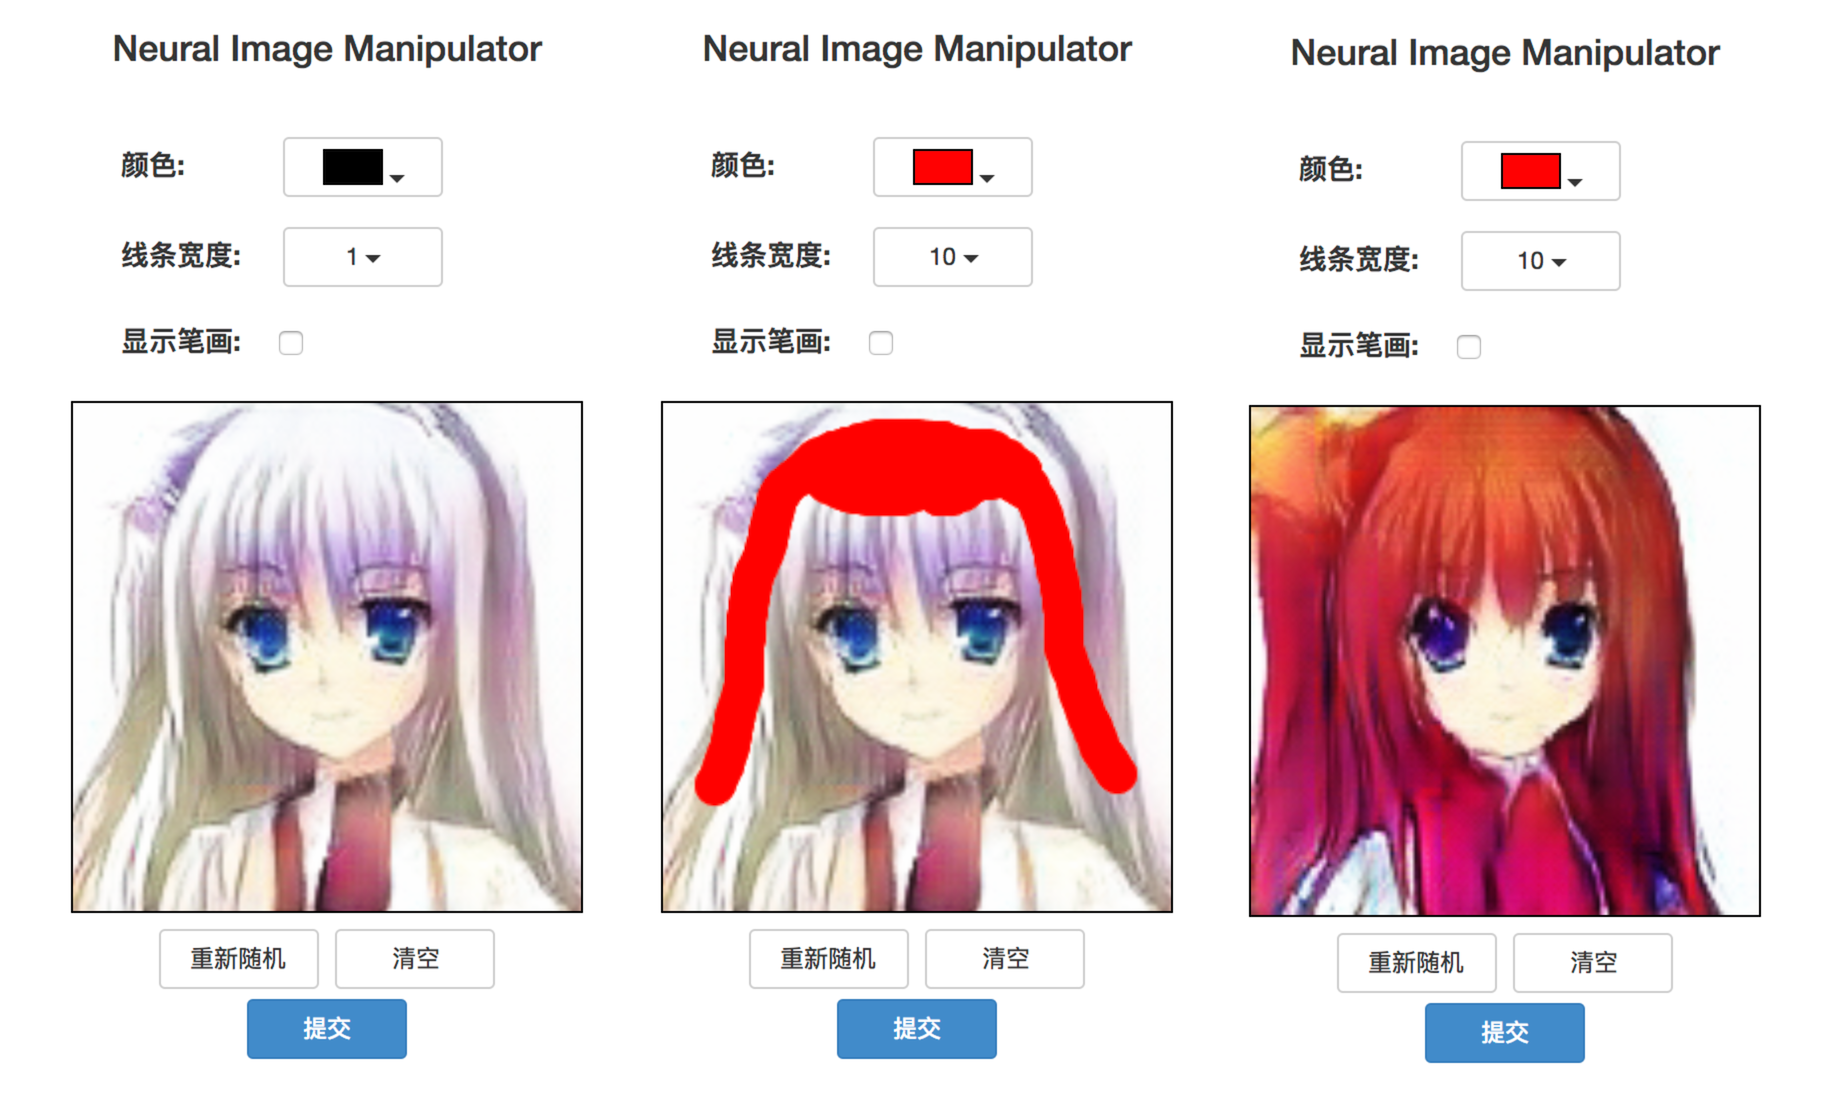
\includegraphics[width=0.9\linewidth]{figs/frontend.png}
  \caption{\kai 项目效果展示。用户通过网页前端绘制简笔画,提交到后台,经过神经网络的优化编辑以后,返回一个符合编辑预期的图像。}
  \label{fig:frontend}
\end{figure}

\section{项目背景}

基于神经网络的图像编辑最早来源于2016提出的交互式生成对抗网络(Interactive Generative Adversarial Network, iGAN)~\cite{Zhu2016Generative}。iGAN提出了基于优化输入的交互式编辑框架,并在户外风景、教堂、鞋子、手提包数据集上进行了实验。iGAN能够做到使得图片随着用户的编辑发生变化,但是它存在着根本的不足,一是生成的质量较低,生成的分辨率仅为 $64\times64$ 而且其内容的真假较易被人分辨;二是在编辑过程中图片的生成质量下滑严重。之后Neural Photo Editor~\cite{Brock2016Neural}的提出改进了生成网络、判别网络,使得在 $64\times64$ 分辨率下的生成质量得到了提升,在人脸编辑领域得到了令人满意的结果。生成质量与编辑质量一直是神经图像编辑的瓶颈,至今仍然处于待解决的状态。尤其是当问题变成了动漫相关的图像子类时,由于此领域内数据集质量的低下,这生成质量与编辑质量的问题变得尤为突出,成为本项目的难点之一。

另外一类与神经图像编辑相关的方法以pix2pix为代表~\cite{isola2016image},通过输入一个精确的语义地图(semantic segmentation map)来产生图像。语义地图指的是一个与原图像大小相等的“地图”,其中每一个像素表明了该像素所属的物体类别。编辑操作通过通过更改输入的语义地图来进行,优点在于生成的质量好于前一种方法,而且其对于物体的形态、边缘有着较高的自由度。它的缺点主要有两点:
\begin{enumerate}
  \item 需要含有语义地图的数据集进行训练,对于数据集的要求非常高,在许多领域上都难以实现。
  \item 这种编辑只能在有限的范围内改动,只能指定某个区域是什么物体,而不能对物体的具体特征进行修改。
\end{enumerate}

基于第二类方法,在插画线稿上色方面有着不错的成果,例如 PaintsChainer\footnote{\url{https://github.com/pfnet/PaintsChainer}} 和 Style2Paint\footnote{\url{https://github.com/pfnet/PaintsChainer}}。这种方法的输入是具有相当美术水准的线稿,输出是上色以后的图像,通过类似于简笔画的方式来对具体的上色进行调节。这种方法的优点继承了pix2pix生成质量较好的优点,但是它只能微调局部的色彩,编辑自由度较低。目前看来这种方法还有另一个应用方面的缺点,它假定了专业人士作为使用者,但是其上色的质量距离专业的水准还有一定距离,使其应用场景有些尴尬。

我们的项目立足于业余用户的简笔画,努力做到面向业余用户的简单而有效的绘图。我们主要与第一类方法进行比较,使用iGAN~\cite{Zhu2016Generative}和NPE~\cite{Brock2016Neural}作为两个基线,其效果如~\ref{fig:baseline1}和~\ref{fig:baseline2}所示。这两种基线方法在各自原文的应用领域上都有着较为令人满意的结果,然而在动漫数据集Getchu上的表现都充分地体现出了其生成质量和编辑质量上的瓶颈。我们的项目针对这个瓶颈提出了有效的解决方法。

\begin{figure}[H]
  \centering
  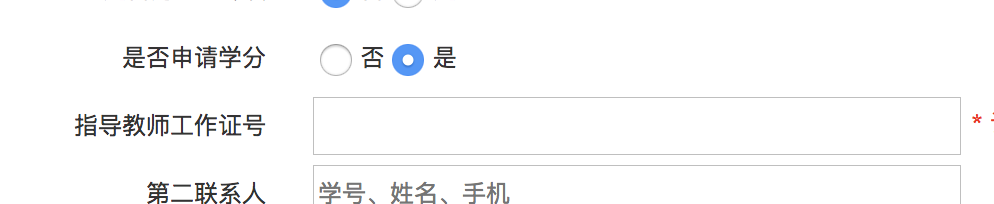
\includegraphics[width=0.9\linewidth]{figs/baseline_shoe.PNG}
  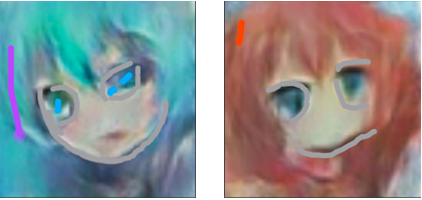
\includegraphics[width=0.9\linewidth]{figs/baseline1.PNG}
  \caption{\kai 基准线1 iGAN~\cite{Zhu2016Generative}的效果。上面的图片来源于原论文,展示了随着用户添加简笔画,鞋子的颜色随之变化的过程,较为符合预期。下面的图片是在Getchu数据集中复现的结果,使用iGAN开源的代码,遵循了原文的设置。图中灰色线条是边缘简笔画,其他的彩色线条是颜色简笔画。经过试验,在编辑图像的过程中图片的真实性频繁下滑。展示的图片经过了精心挑选,达到了iGAN所能达到的最佳效果,但仍然十分不美观。}
  \label{fig:baseline1}
\end{figure}

\begin{figure}[H]
  \centering
  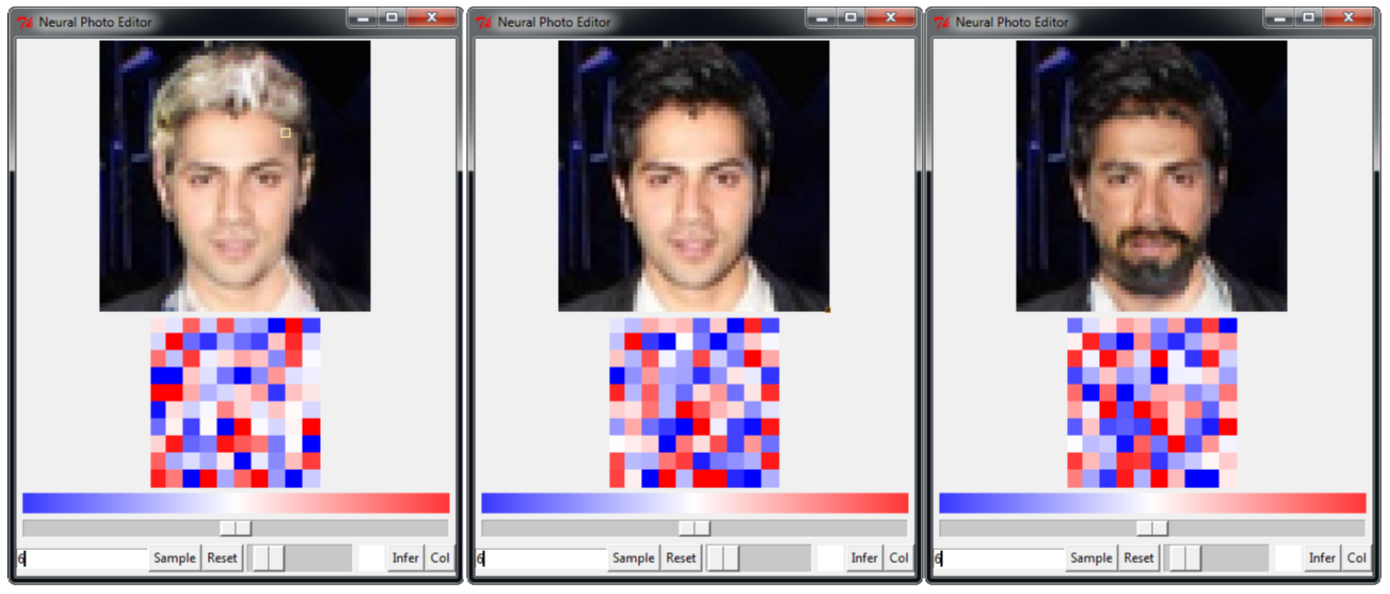
\includegraphics[width=0.7\linewidth]{figs/baseline_face.PNG}
  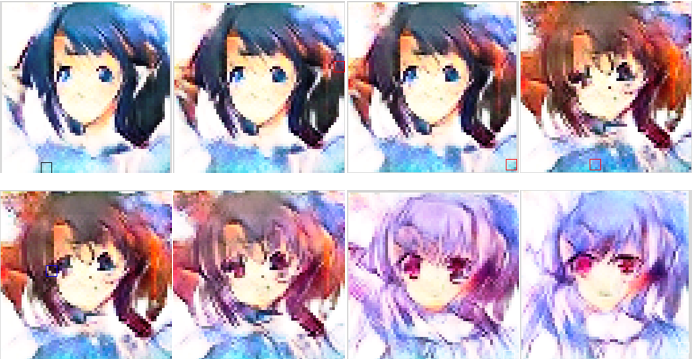
\includegraphics[width=0.9\linewidth]{figs/baseline2.PNG}
  \caption{\kai 基准线2 NPE~\cite{Brock2016Neural}的效果。上面的图片来源于原论文,中间的图片是原图片,左右分别是经过编辑的图片。下面的图片是NPE在Getchu数据集上的复现,使用了NPE开源的代码,遵循了原文的设置。从左上到右下是在神经图像编辑过程中顺序产生的,用户在$1\sim5$张中头发的位置画了红色线条,在 $6\sim8$张中画了蓝色线条(线条未显示)。头像颜色变化基本与预期相符,体现了编辑的有效性,但是生成的质量和编辑的稳定性不令人满意。}
  \label{fig:baseline2}
\end{figure}

\section{核心技术}

完成神经图像编辑的核心技术分为两部分:网络的训练和图像编辑框架。在网络训练中,我们参考了~\cite{Jin2017Towards}的网络设计了自己的生成网络和判别网络。在图像编辑的框架中,我们参考了第一类神经图像编辑中优化输入的方法,对其进行了改进。

\subsection{图像编辑}

\begin{figure}[H]
  \centering
  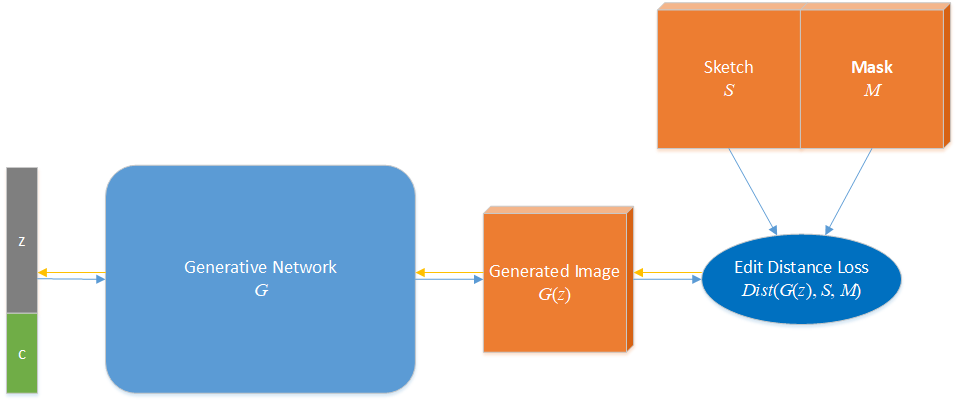
\includegraphics[width=1\linewidth]{figs/workflow1.png}
  \caption{\kai 编辑图像的实现方法。此时生成网络已经训练完成,从随机向量出发,由生成网络生成初始图像,用户给定简笔画和对应的遮罩,由编辑距离函数计算误差和导数,使用梯度下降更新 $z$,产生一张新的、与草图相似的图片,达到编辑图像的目的。蓝箭头表示数据流向,橙色箭头表示导数。}
  \label{fig:workflow1}
\end{figure}

我们使用训练好的生成网络$G$实现对于图像的编辑工作。

一个生成网络$G(z, c)$接受随机向量$z$(遵循高斯分布)和条件向量$c$作为输入,生成图像$I = G(z, c)$。同时用户给定编辑图像$I'$,例如一副简笔画,则可以据此给出生成图像与编辑图像之间的距离$Dist(G(z, c), I')$。设$I$在像素点$(i, j)$处的RGB颜色向量为$I_{ij}$。设$M_{ij}$为像素点$(i, j)$处的遮罩向量,含义是用户编辑的部分是否包含像素点$(i, j)$。$M_{ij}$的值只可能为全$0$或全$1$,定义如下:
%
\begin{align}
  M_{ij} =
  \begin{cases}
    [0, 0, 0],   &  \text{$\norm{I'_{ij}} = 0$} \\
    [1, 1, 1],   &  \text{$\norm{I'_{ij}} \neq 0$}
  \end{cases}
\end{align}
%
则我们可以基于已有的$M_{ij}$、$I_{ij}$和$I'_{ij}$定义原生成图像与编辑图像之间的距离,这里的距离定义为两幅图中每个用户编辑的像素点距离的 L1-norm 除以一个合理的代表用户修改总点数的值。这样定义的目的是为了仅仅对用户编辑的位置进行修改,且提供与修改像素点数无关的距离函数,避免用户修改的点过少时效果变差。即定义
%
\begin{align}
  Dist(I, I') = \frac{\sum_{ij} |(I_{ij} - I'_{ij}) \cdot M_{ij}|}{1 + \sum_{ij} \frac{|M_{ij}|}{\sqrt 3}}
\end{align}
%
假设 $G$ 已经得到,本文的基本目标是求使$Dist(G(z, c), I')$最小的$z$和$c$,即
%
\begin{align}
  \arg\min_{z, c} Dist(G(z, c), I')
\end{align}
%
为求这样的$z$和$c$,先给出随机的合法初值$z_{0}$和$c_{0}$,再将距离函数对$z_{0}$和$c_{0}$求偏导:
%
\begin{align}
  \Delta z_{0} & = \frac{\partial}{\partial z} Dist(G(z_{0}, c_{0}), I') \\
  \Delta c_{0} & = \frac{\partial}{\partial c} Dist(G(z_{0}, c_{0}), I')
\end{align}
%
之后,在$z$和$c$的反函数域上以学习率$lr$使用梯度下降(Gradient Descent)算法进行学习,并限制$\tilde z_{1}$和$\tilde c_{1}$在合法的边界中:
%
\begin{align}
  \tilde z_{1} & = \mathrm{arctanh}(z_{0}) - lr \cdot \Delta z_{0} \\
  \tilde c_{1} & = - \log \left(\frac{1}{c_{0}} - 1\right) - lr \cdot \Delta c_{0}
\end{align}
%
最后,将$\tilde z_{1}$和$\tilde c_{1}$变换回原来的函数域,得到新的值$z_{1}$和$c_{1}$:
%
\begin{align}
  z_{1} & = \tanh (\tilde z_{1}) \\
  c_{1} & = \sigma(\tilde c_{1})
\end{align}
%
其中 $\sigma$ 为 sigmoid 函数。重复这样的学习,即可使$Dist(G(z, c), I')$不断减小,直到生成符合要求的图片。

\subsection{网络训练}

本项目中对于多种网络结构和训练方法进行了尝试,最终确定了和~\cite{Jin2017Towards}类似的网络结构与训练方法。我们采用了使用多层Residual Block ~\cite{he2016deep} 搭建的深层生成器和判别器,使用DRAGAN ~\cite{kodali2017convergence}加上辅助分类器~\cite{odena2016conditional}的训练方法进行。

设真实数据集为$D_R$,一个训练样例可以表示成$x \sim P_{data}$。生成器接受随机向量 $z$ 和条件向量 $c$ 的输入,且$z \sim P_{noise}$,$c \sim P_{cond}$,$P_{cond}$ 表示给定标签下的先验分布。$\mathcal{L}_{adv}$,$\mathcal{L}_{gp}$ 和 $\mathcal{L}_{reg}$ 分别表示 adversarial,gradient penalty 和 weight regularization 的 损失函数系数。

使用DRAGAN的训练可以用如下公式表达:
%
\begin{align}
  \mathcal{L}_{adv}(D) &= -\mathbb{E}_{x\sim P_{data}}[\log D(x)] - \mathbb{E}_{z\sim P_{noise},c\sim P_{cond}}\big[\log(1-D(G(z,c)))\big] \\
  \mathcal{L}_{cls}(D) &= \mathbb{E}_{x\sim P_{data}}\big[\log P_D[label_x|x]\big] + \mathbb{E}_{x\sim P_{noise},c\sim P_{cond}}\Big[\log\big(P_D[c|G(z,c)]\big)\Big] \\
  \mathcal{L}_{gp}(D) &= \mathbb{E}_{\tilde{x}\sim P_{perturebed\_data}}\left[\big(\norm{\nabla_{\tilde{x}}D(\tilde{x})}_2-1\big)^2\right] \\
  \mathcal{L}_{adv}(G) &= \mathbb{E}_{x\sim P_{noise},c\sim P_{cond}}\big[\log D(G(z,c))\big] \\
  \mathcal{L}_{cls}(G) &= \mathbb{E}_{x\sim P_{noise},c\sim P_{cond}}\big[\log P_D[c|G(z,c)]\big] \\
  \mathcal{L}_{DRAGAN}(D) &= \mathcal{L}_{cls}(D) + \lambda_{adv}\mathcal{L}_{adv}(D) + \lambda_{gp}\mathcal{L}_{gp}(D) + \lambda_{reg} \mathcal{L}_{2}(D) \\
  \mathcal{L}_{DRAGAN}(G) &= \lambda_{adv}\mathcal{L}_{adv}(G) + \mathcal{L}_{cls}(G) + \lambda_{reg} \mathcal{L}_{2}(D)
\end{align}
%
其中$\mathcal{L}_{2}$是L2正则化损失,$\tilde{x}$是经过扰动的真实数据($\sigma_x$ 为 $x$ 的标准差),
%
\begin{align}
  \tilde{x} & = x + \frac{1}{2}\alpha\sigma_x \\
  \alpha & \sim U(0, 1)
\end{align}

使用Adam~\cite{Kingma2014Adam}优化器迭代交替优化$\mathcal{L}_{DRAGAN}(D)$,$\mathcal{L}_{DRAGAN}(G)$完成训练。

% [TODO]: Network structure

\subsubsection{演示模型的训练}

最终我们确定的训练设置是:Adam~\cite{Kingma2014Adam}优化器以$2 \times 10^{-4}$的初始学习率进行$5 \times 10^{4}$的迭代,然后在接下来$5 \times 10^{4}$的迭代中线性降低学习率至$1 \times 10^{5}$。网络使用128维的随机向量$z$和34维的条件向量$c$,前者服从$\sigma=1, \mu=0$的正态分布,后者在保证类互斥条件下由均匀分布随机产生。各个loss的系数是$\lambda_{gp}=0.5$,$\lambda_{reg}=10^{-4}$,$\lambda_{adv}=1$。$\mathrm{batchsize}=64$。训练在Titan X GPU下需要花费大约20小时的时间。

图~\ref{fig:goodmodel_dragan}~展示了我们使用的演示模型的训练loss变化:

\begin{figure}[H]
  \centering
  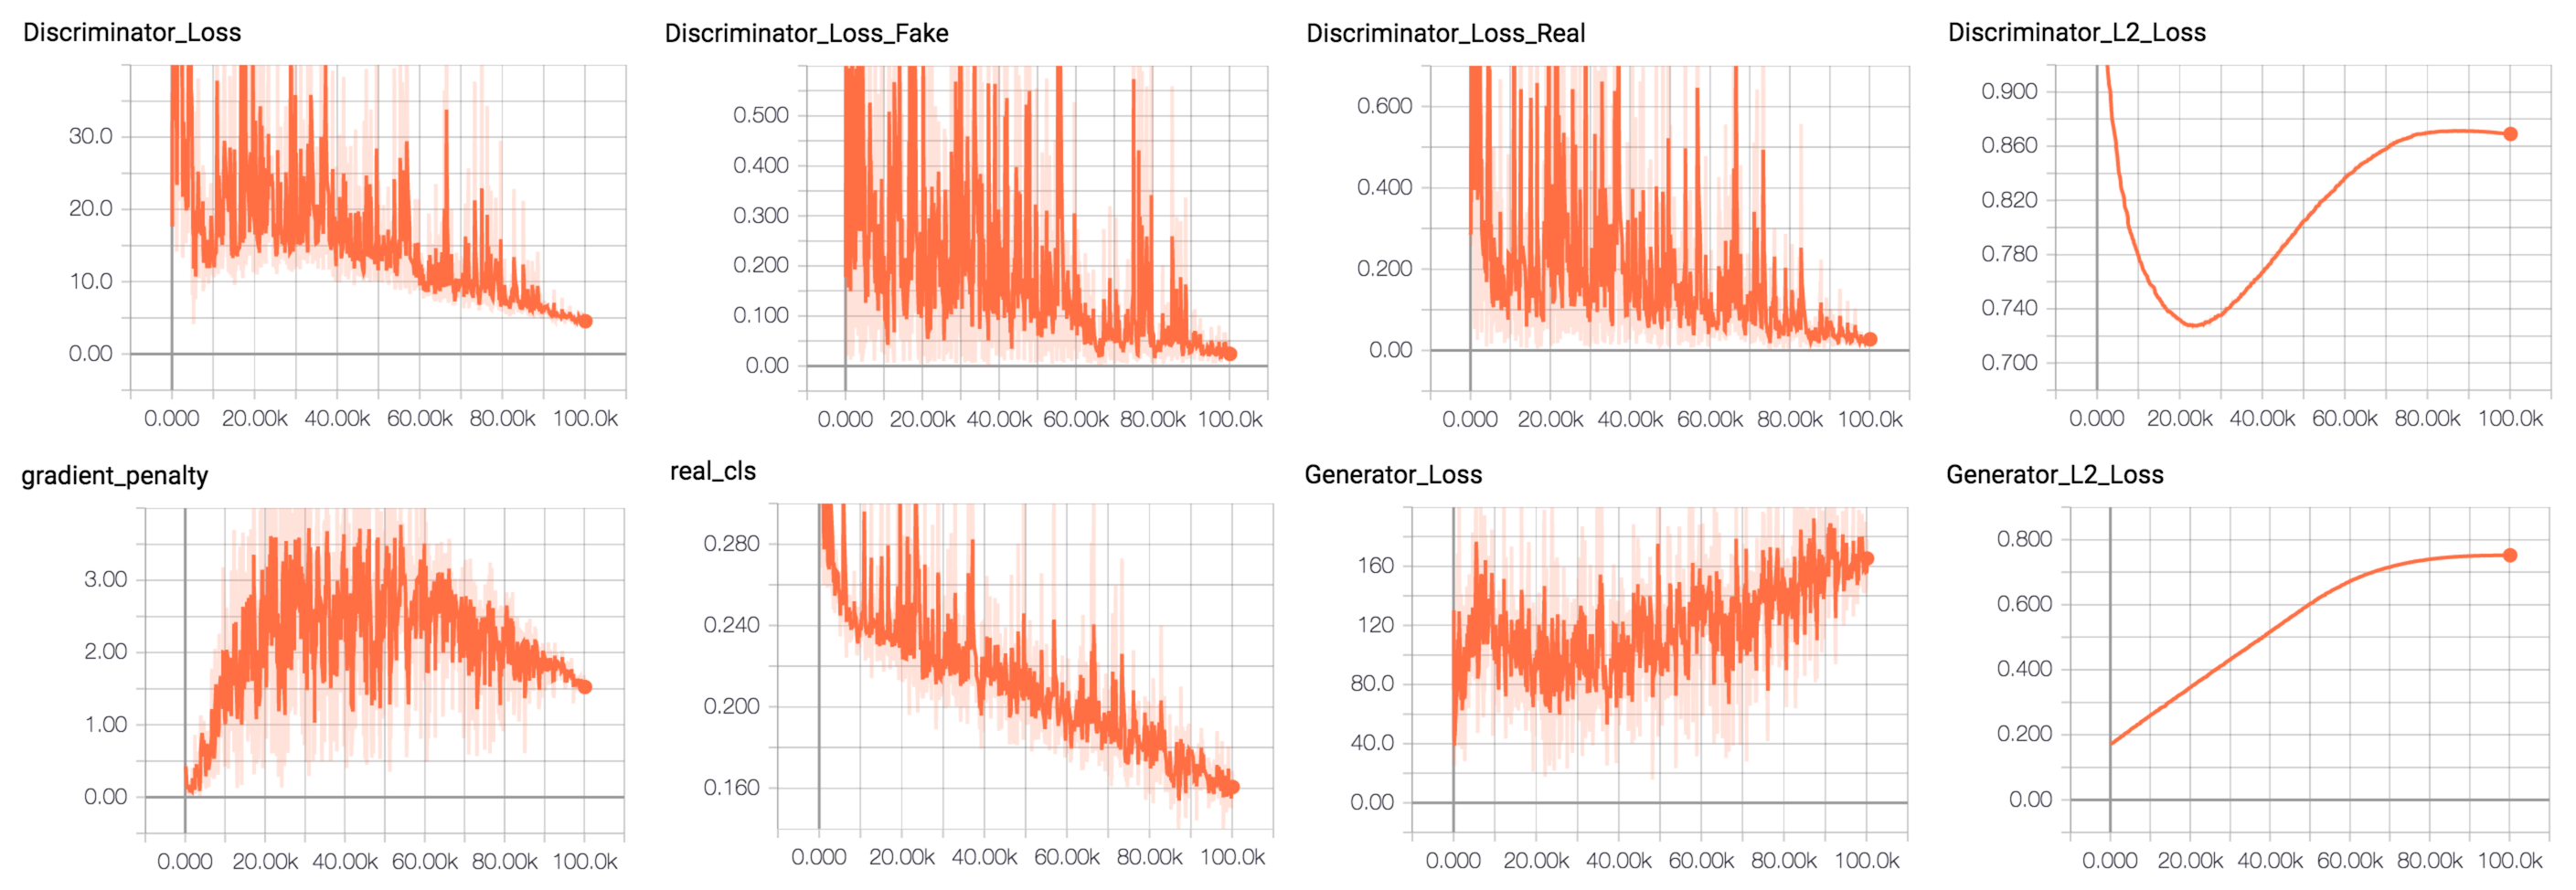
\includegraphics[width=1\linewidth]{figs/good_model_dragan.png}
  \caption{\kai 演示模型的训练loss图。左上角开始的Discriminator Loss是判别器的总损失,其右的Fake和Real损失分别是判别器识别生成图片和真实图片的损失。左下角的gradient penalty如上文所述,其右是判别器分类图片的交叉熵损失。再右边是Generator Loss的总损失,最右边是两个网络的正则损失。}
  \label{fig:goodmodel_dragan}
\end{figure}

可以看出生成器的损失除了刚刚开始的震荡较为剧烈以外,整体在稳步下降。查看固定随机数的生成结果,如图~\ref{fig:dragan_evolve}~所示。从每一个随机种子生成的图片可以看到生成的不断完善、生成结果质量的稳定上升。

\begin{figure}[H]
  \centering
  \includegraphics[width=1\linewidth]{figs/good_model_dragan_sample.png}
  \caption{\kai 演示模型的训练中生成图像的演化。从左到右四张图片分别是25k, 50k, 75k, 100k迭代时的生成结果。每一张图片包含16个固定随机数生成的结果。}
  \label{fig:dragan_evolve}
\end{figure}

\subsection{数据集}

我们使用的数据集取自 Getchu\footnote{\url{http://getchu.com}}网站,该网站汇聚了大量高质量动漫人物立绘,且图片中仅有单人,背景为白色,很适合作为我们的训练数据。

我们使用爬虫工具从该网站上获得了 22000 张图片,经过 OpenCV \footnote{\url{https://opencv.org}}识别人脸,然后裁剪、缩放到 $128\times128$大小。

\begin{figure}[H]
  \centering
  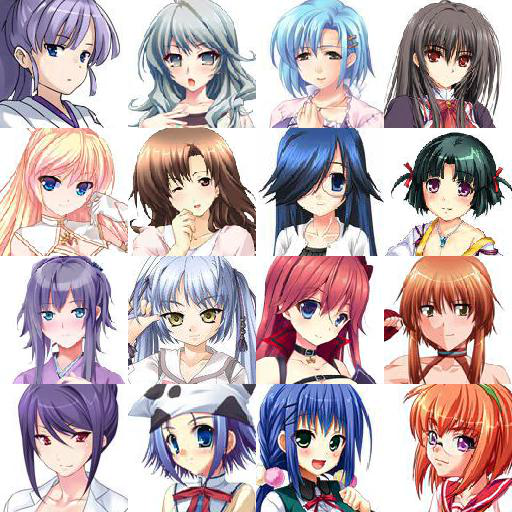
\includegraphics[width=0.5\linewidth]{figs/ex6.png}
  \caption{\kai Getchu数据集。采用 OpenCV 识别人脸,经过裁剪、缩放到 $64\times64$ 的大小。}
  \label{fig:getchu_disp}
\end{figure}

然后,我们对采集到的图像使用 illustration2vec~\cite{Saito2015Illustration2Vec}进行分类,可得到每张图片属于某一类别的概率(illustration2vec有512个类别)。选取其中与我们的任务相关的 10 个 大类 和 34 个小类,可编码一个 34 维的向量,即条件向量 $c$,如表~\ref{table:ill_c}~所示。向量的第$i$维取值为 0 或 1,如果是 1 表示该图片具有编号为 $i$ 的特征,且同一大类的各个子类中最多只能有一个 1。

\renewcommand{\multirowsetup}{\centering}
\begin{table}[H]
  \centering
  \begin{tabular}{|C{0.8cm}|C{1.1cm}|C{1.1cm}|C{1.1cm}|C{1.1cm}|C{1.1cm}|C{1.1cm}|C{1.1cm}|C{1.1cm}|}
    \hline
    编号   & 0 & 1 & 2 & 3 & 4 & 5 & 6 & 7 \\ \hline
    \multirow{2}{*}{类别} & \multicolumn{8}{c|}{发色}  \\ \cline{2-9}
          & 金色 & 棕色 & 黑色 & 蓝色 & 粉色 & 紫色 & 绿色 & 红色 \\ \hline
    \hline
    编号   & 8 & 9 & 10 & 11 & 12 & 13 & 4 & 15 \\ \hline
    \multirow{2}{*}{类别} & \multicolumn{5}{c|}{发色} & \multicolumn{2}{c|}{发长} & 发型 \\ \cline{2-9}
          & 银色 & 白色 & 橙色 & 天蓝色 & 灰色 & 长发 & 短发 & 双马尾\\ \hline
    \hline
    编号   & 16 & 17 & 18 & 19 & 20 & 21 & 22 & 23 \\ \hline
    \multirow{2}{*}{类别}   & \multicolumn{2}{c|}{发型} & \multirow{2}{1.1cm}{是否脸红} & \multirow{2}{1.1cm}{是否微笑} & \multirow{2}{1.1cm}{是否张嘴} & \multirow{2}{1.1cm}{是否戴帽子} & \multirow{2}{1.1cm}{是否有缎带} & \multirow{2}{1.1cm}{是否戴眼镜} \\ \cline{2-3}
          & 卷发 & 马尾 &  &  &  &  & & \\ \hline
    \hline
    编号   & 24 & 25 & 26 & 27 & 28 & 29 & 30 & 31 \\ \hline
    \multirow{2}{*}{类别} & \multicolumn{8}{c|}{眼睛颜色}  \\ \cline{2-9}
          & 蓝色 & 红色 & 棕色 & 绿色 & 紫色 & 黄色 & 粉色 & 天蓝色 \\ \hline
    \hline
    编号   & 32 & 33 &  \multicolumn{6}{c|}{} \\ \hline
    \multirow{2}{*}{类别} & \multicolumn{2}{c|}{眼睛颜色} & \multicolumn{6}{c|}{} \\ \cline{2-3}
          & 黑色 & 橙色 & \multicolumn{6}{c|}{}\\ \hline
  \end{tabular}\newline
  \caption{\kai 条件向量的构成。共有 10 个大类和 34 个小类,向量值的某一维为 1,表示具有该维所对应的那个类别的特征。}\label{table:ill_c}
\end{table}

\section{效果展示}

\begin{figure}[H]
  \centering
  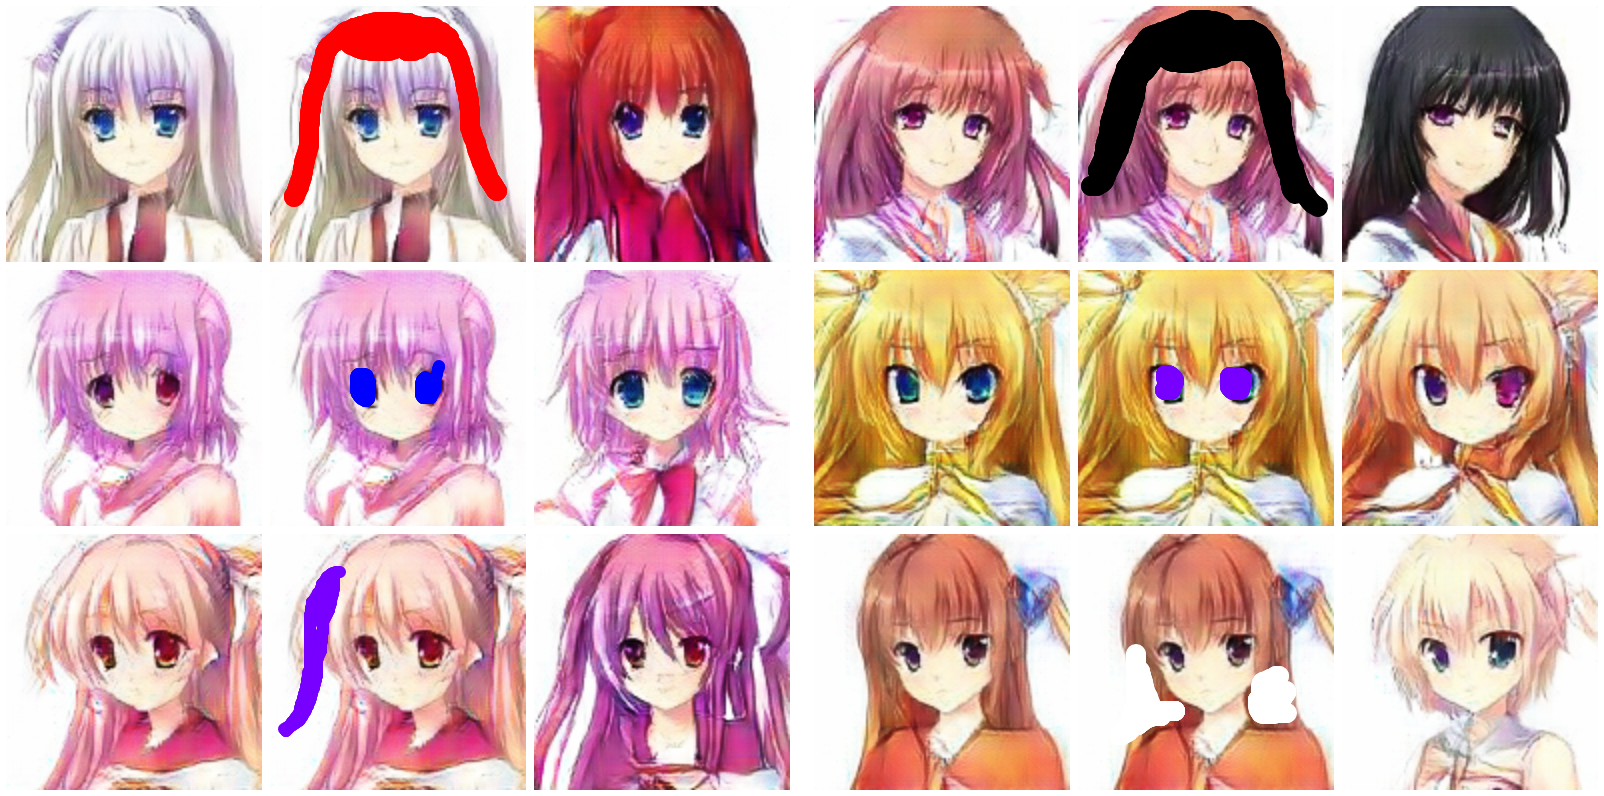
\includegraphics[width=0.9\linewidth]{figs/pic.png}
  \caption{\kai 动漫人脸编辑效果展示,共六组,每组三幅图。每组中,左中右分别为原图、原画加上简笔画图、结果图。第一行为成功更换发色的例子,第二行为成功更换瞳色的例子,第三行为成功更换发型的例子。与两种基线方法相比,在生成质量、编辑稳定性、编辑自由度上都有着显著的提升。}
  \label{fig:comic}
\end{figure}

% [TODO]: caption of shoe & handbag by KMY

\begin{figure}[H]
  \centering
  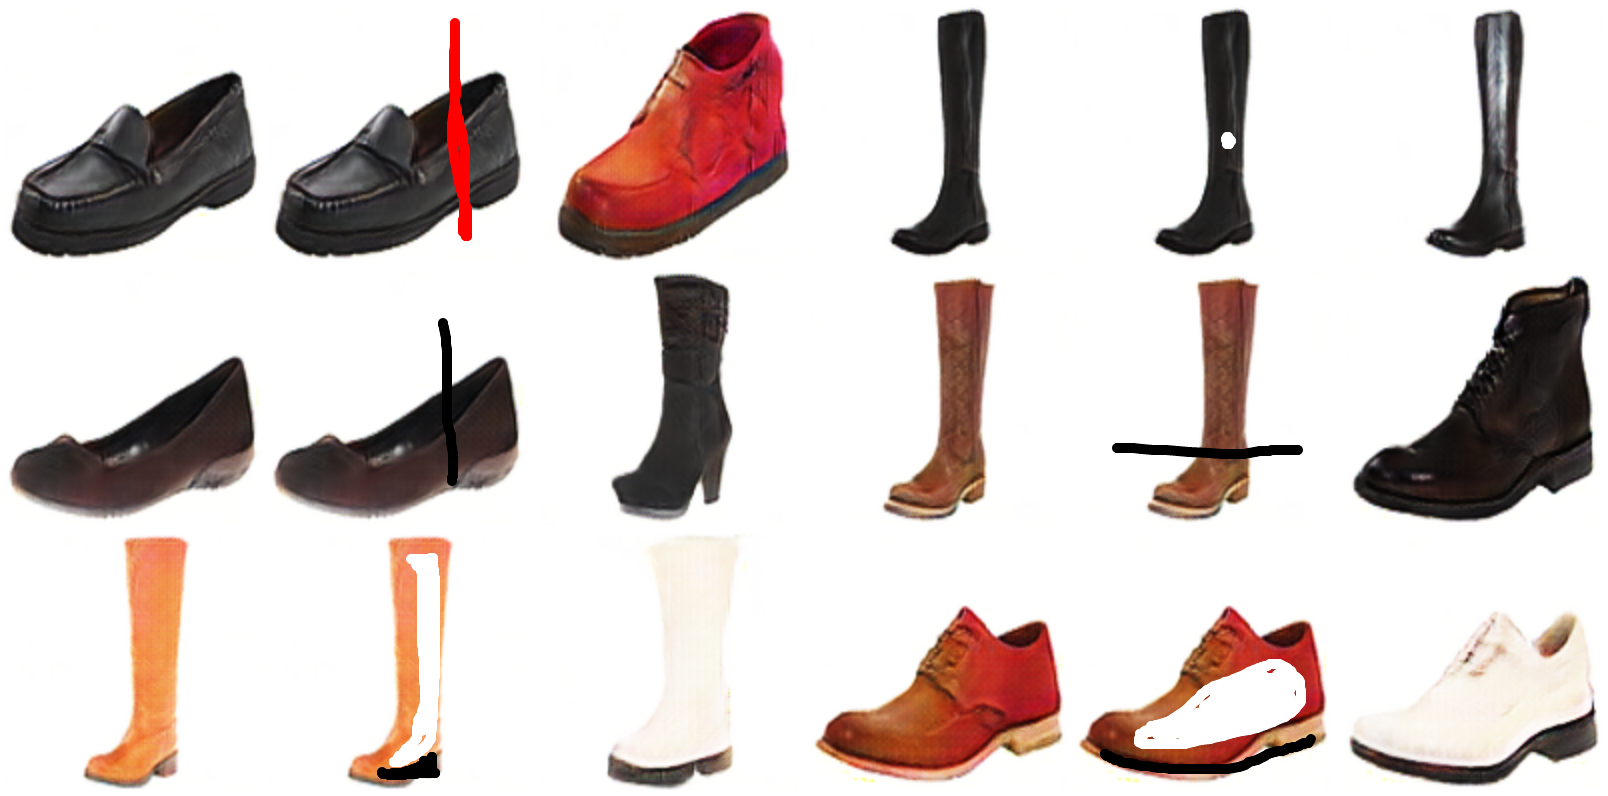
\includegraphics[width=0.9\linewidth]{figs/shoes.png}
  \caption{\kai 鞋子图片编辑效果展示,共六组,每组三幅图。每组中,左中右分别为原画、原画加上简笔画图、结果图。第一行为成功更换鞋子颜色的例子,第二行为成功更换鞋子样式的例子,第三行为成功将鞋子变为双色的例子。}
  \label{fig:shoe}
\end{figure}

\begin{figure}[H]
  \centering
  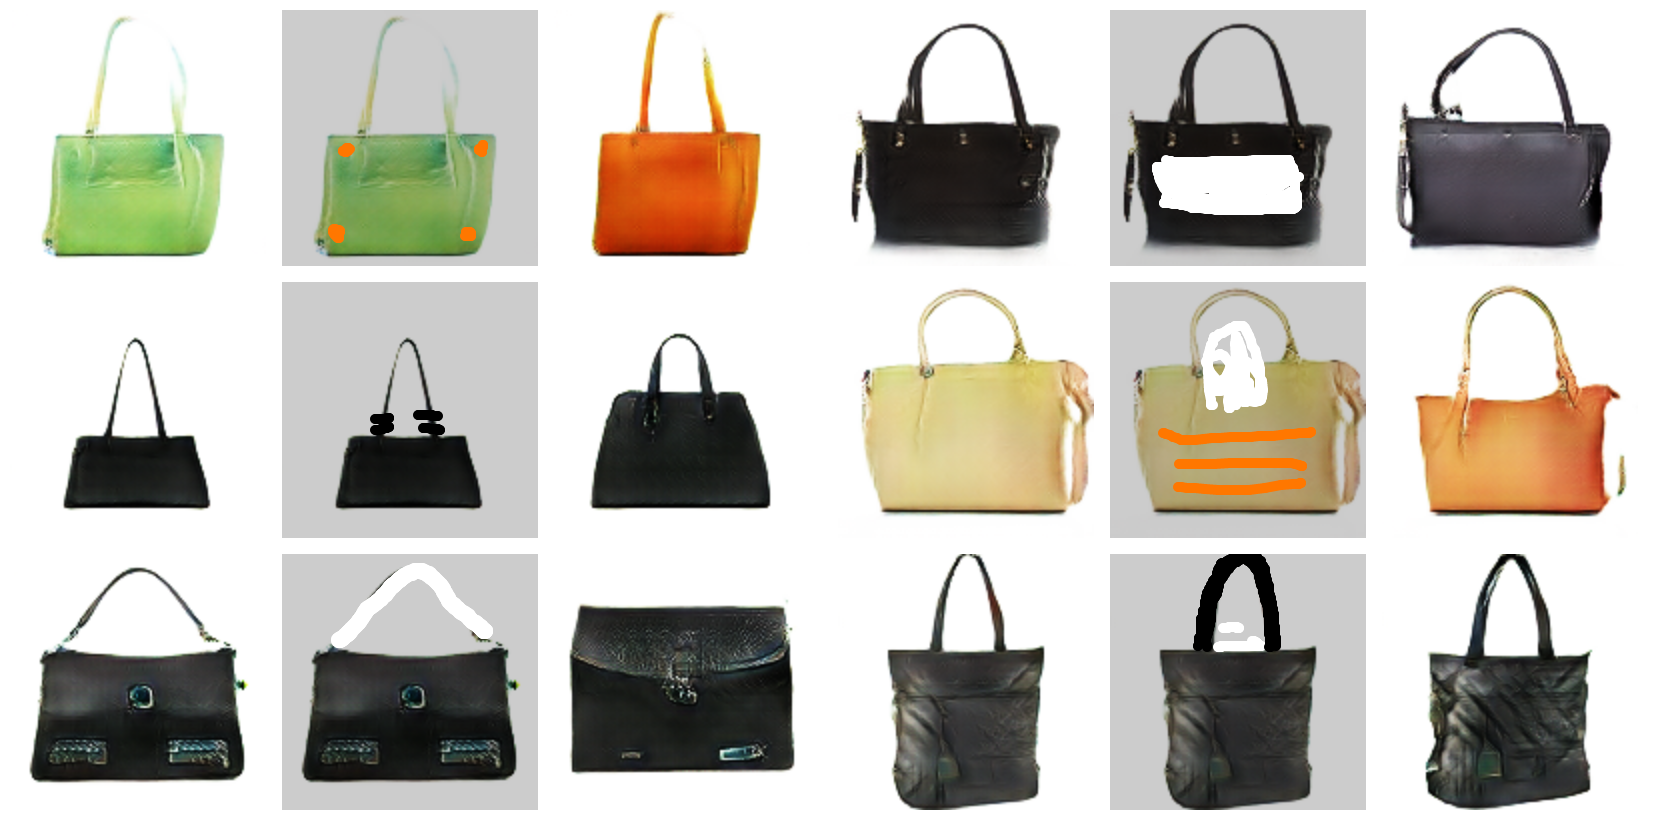
\includegraphics[width=0.9\linewidth]{figs/handbags.png}
  \caption{\kai 手提包图片编辑效果展示,共六组,每组三幅图。每组中,左中右分别为原画、原画加上简笔画图、结果图。第一行为成功更换手提包颜色的例子,第二行为成功调整手提包大小的例子,第三行为成功修改手提包带子的例子。}
  \label{fig:handbag}
\end{figure}

将编辑操作应用于训练好的网络,我们得到了效果优秀的图像生成和编辑效果。如图~\ref{fig:comic}~所示,我们的模型能够生成高质量的图片,并对其进行稳定的编辑,在编辑过程中不容易丧失图片的真实性。同时编辑支持多种功能,眼睛、头发的颜色,发型等可以按照简笔画给定的方式变化。

在图~\ref{fig:comic}~中,第一行的两组为更换发色的例子,第二行的两组为更换瞳色的例子,第三行的两组为更换发型的例子。可以看出,第一行中,左边的一组成功将原图中的人物的发色从白色变成了红色,而右边的一组成功将原图中的人物的发色从红色变成了黑色。第二行中,左边的一组成功将人物瞳色从红色变成了蓝色,而右边的一组将人物瞳色从蓝色变成了紫红色。第三行中,左边的一组成功在人物头上添加了一束紫色的头发,而右边的一组成功去掉了人物头两侧的头发,将人物从长发变成了短发。

在图~\ref{fig:shoe}~中,第一行的两组为更换鞋子颜色的例子,第二行的两组为更换鞋子样式的例子,第三行的两组为将鞋子变为双色的例子。可以看出,第一行中,左边的一组成功将原图中鞋子的颜色从棕色变成了黄色,而右边的一组成功将原图中的黑色鞋子加上了光泽。第二行中,左边的一组成功将原图中的平底鞋变成了高跟靴子,而右边的一组将原图中的棕色长筒靴变成了黑色高帮靴子。第三行中,左边的一组成功将原图中的棕色长筒靴变为了黑底白色的靴子,右边的一组成功将红色的皮鞋变成了白底黑色,实现了将鞋子变为双色的过程。

在图~\ref{fig:handbag}~中,第一行的两组为更换手提包颜色的例子,第二行的两组为更换手提包大小的例子,第三行的两组为修改手提包带子的例子。可以看出,第一行中,左边的一组成功将原图中手提包的颜色从绿色变成了橙色,而右边的一组成功将原图中的黑色手提包加上了光泽。第二行中,左边的一组成功将原图中的手提包变大,而右边的一组将原图中的黄色手提包变成了橙色,且将手提包变小。第三行中,左边的一组成功将原图中的手提包的带子去掉,右边的一组成功将手提包的带子加粗。

可以看出,我们生成的模型可以进行对动漫人物的发色、瞳色、发型等多方面特征进行编辑,对鞋子的颜色、样式、光泽等多方面特征进行编辑,对手提包的颜色、大小、带子等多方面特征进行编辑,且效果出色。与基线相比,生成质量上升,生成清晰度上升,编辑稳定性提高,编辑多样性也有提高。

\subsection{网页应用}

我们基于训练好的模型,开发了一个基于 B/S 架构的网页应用,可以通过 Web 浏览器进行在线图像编辑。

\subsubsection{网页端}
我们的网页端界面如图 \ref{figure:web1} $\sim$ 图 \ref{figure:web3}  所示,能够运行在任何一款现代浏览器上。

\begin{figure}[H]
  \begin{minipage}[t]{0.33\linewidth}
      \centering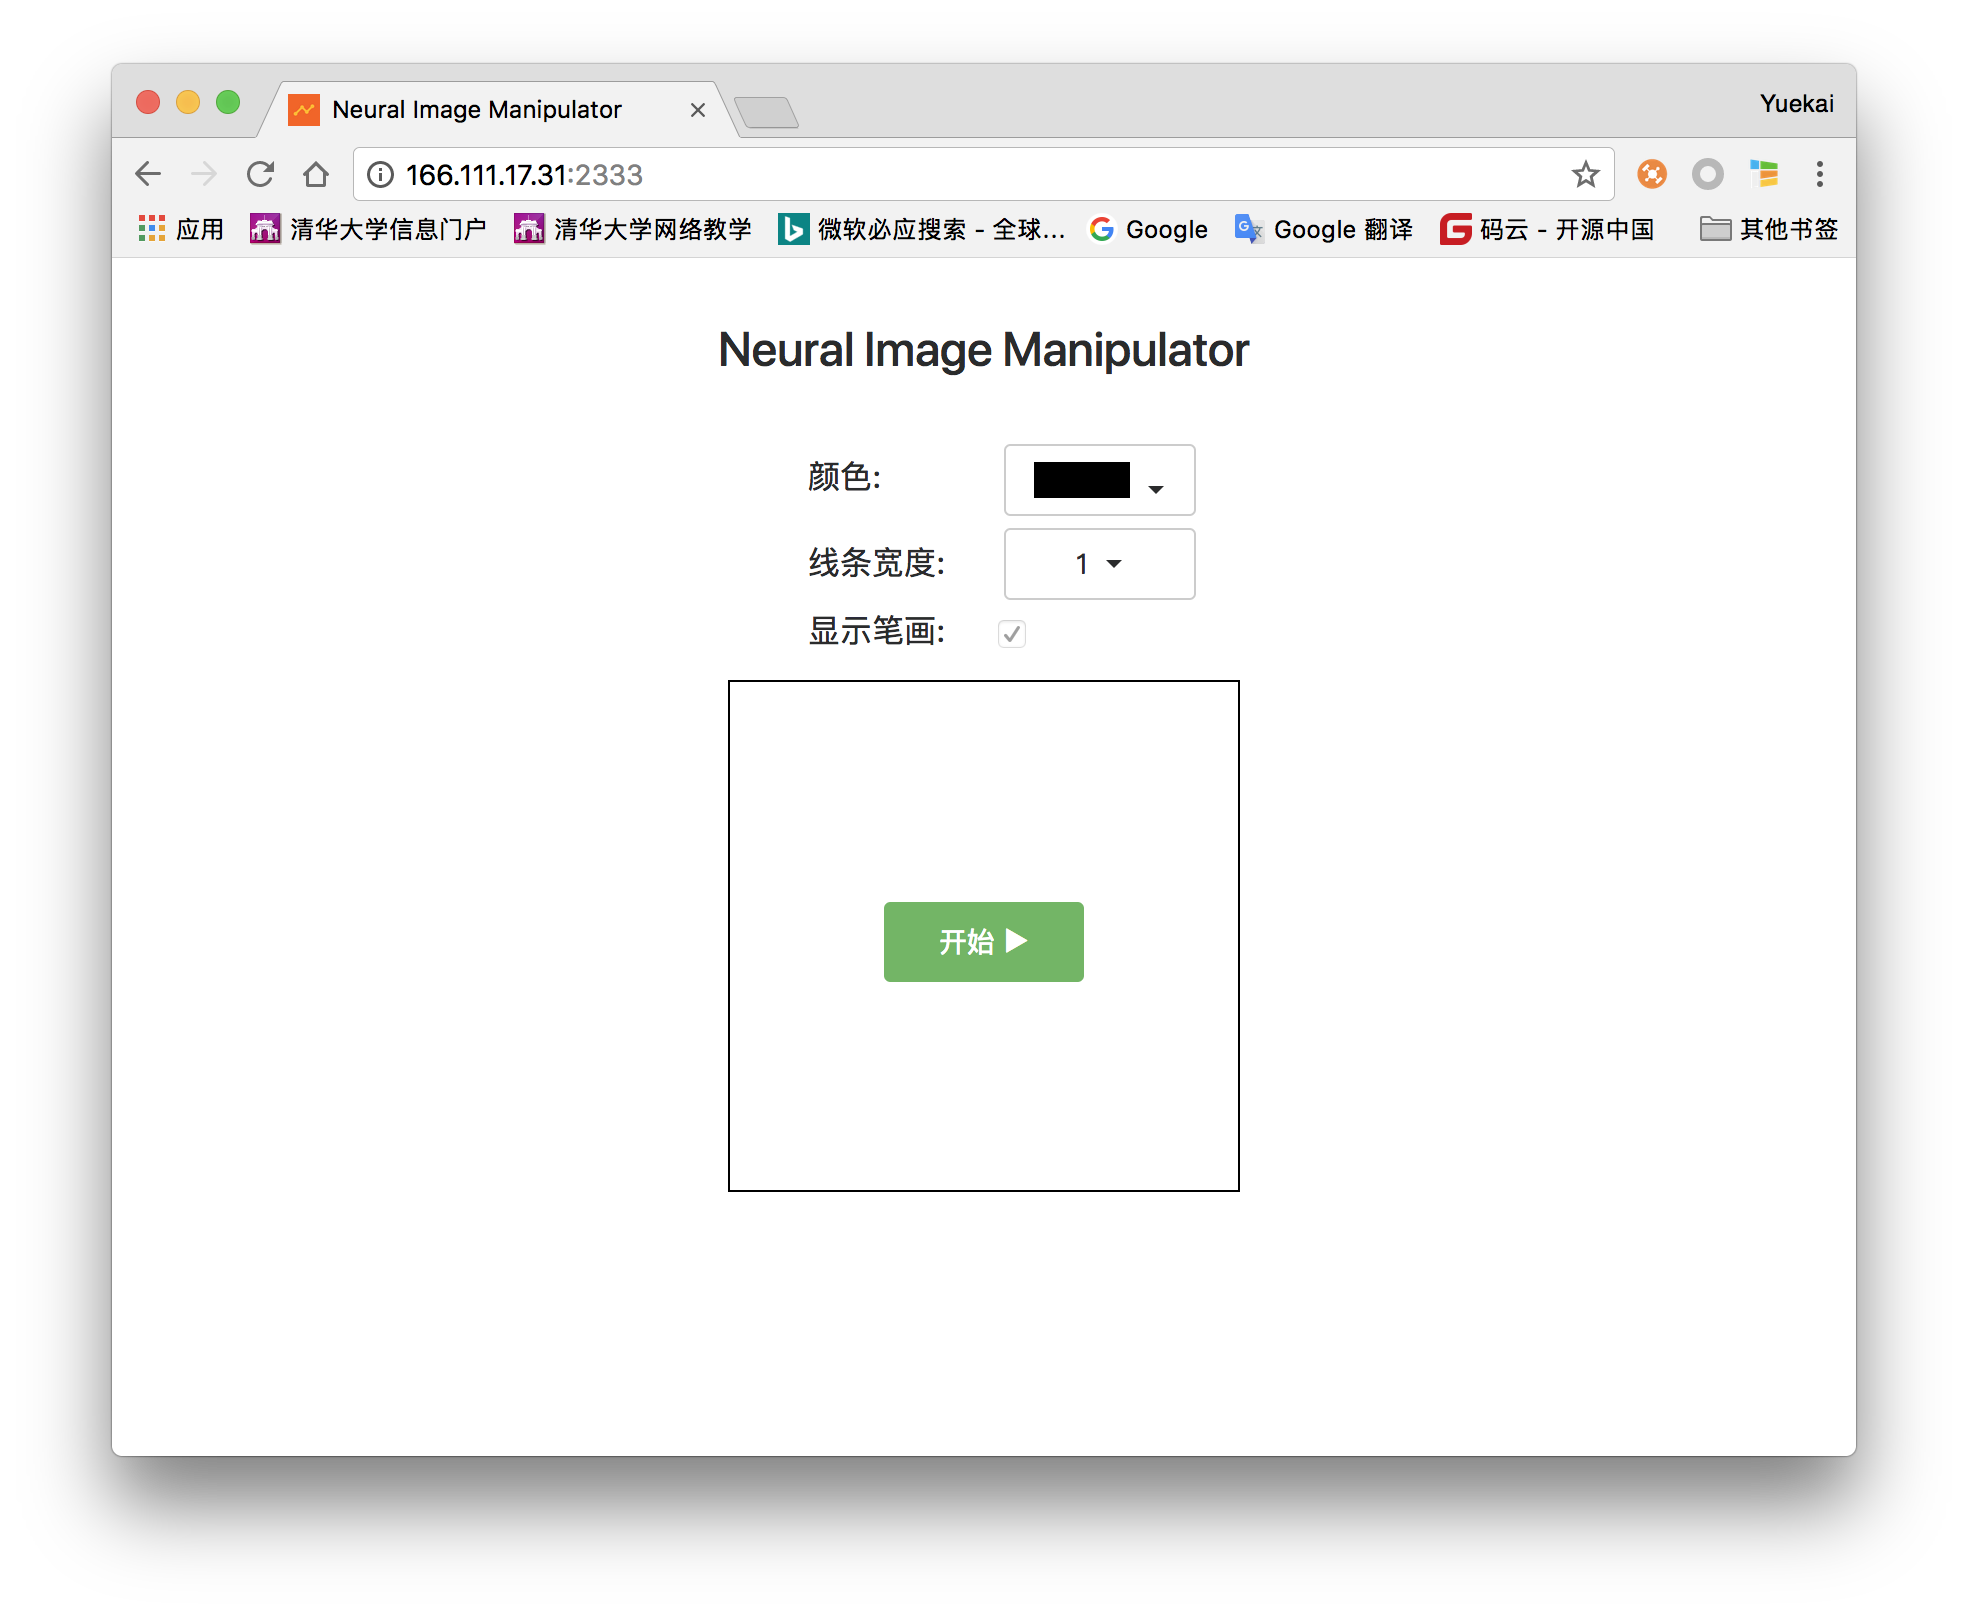
\includegraphics[height=4cm]{figs/web1.png}
      \caption{\kai 开始页面}\label{figure:web1}
  \end{minipage}%
  \begin{minipage}[t]{0.33\linewidth}
      \centering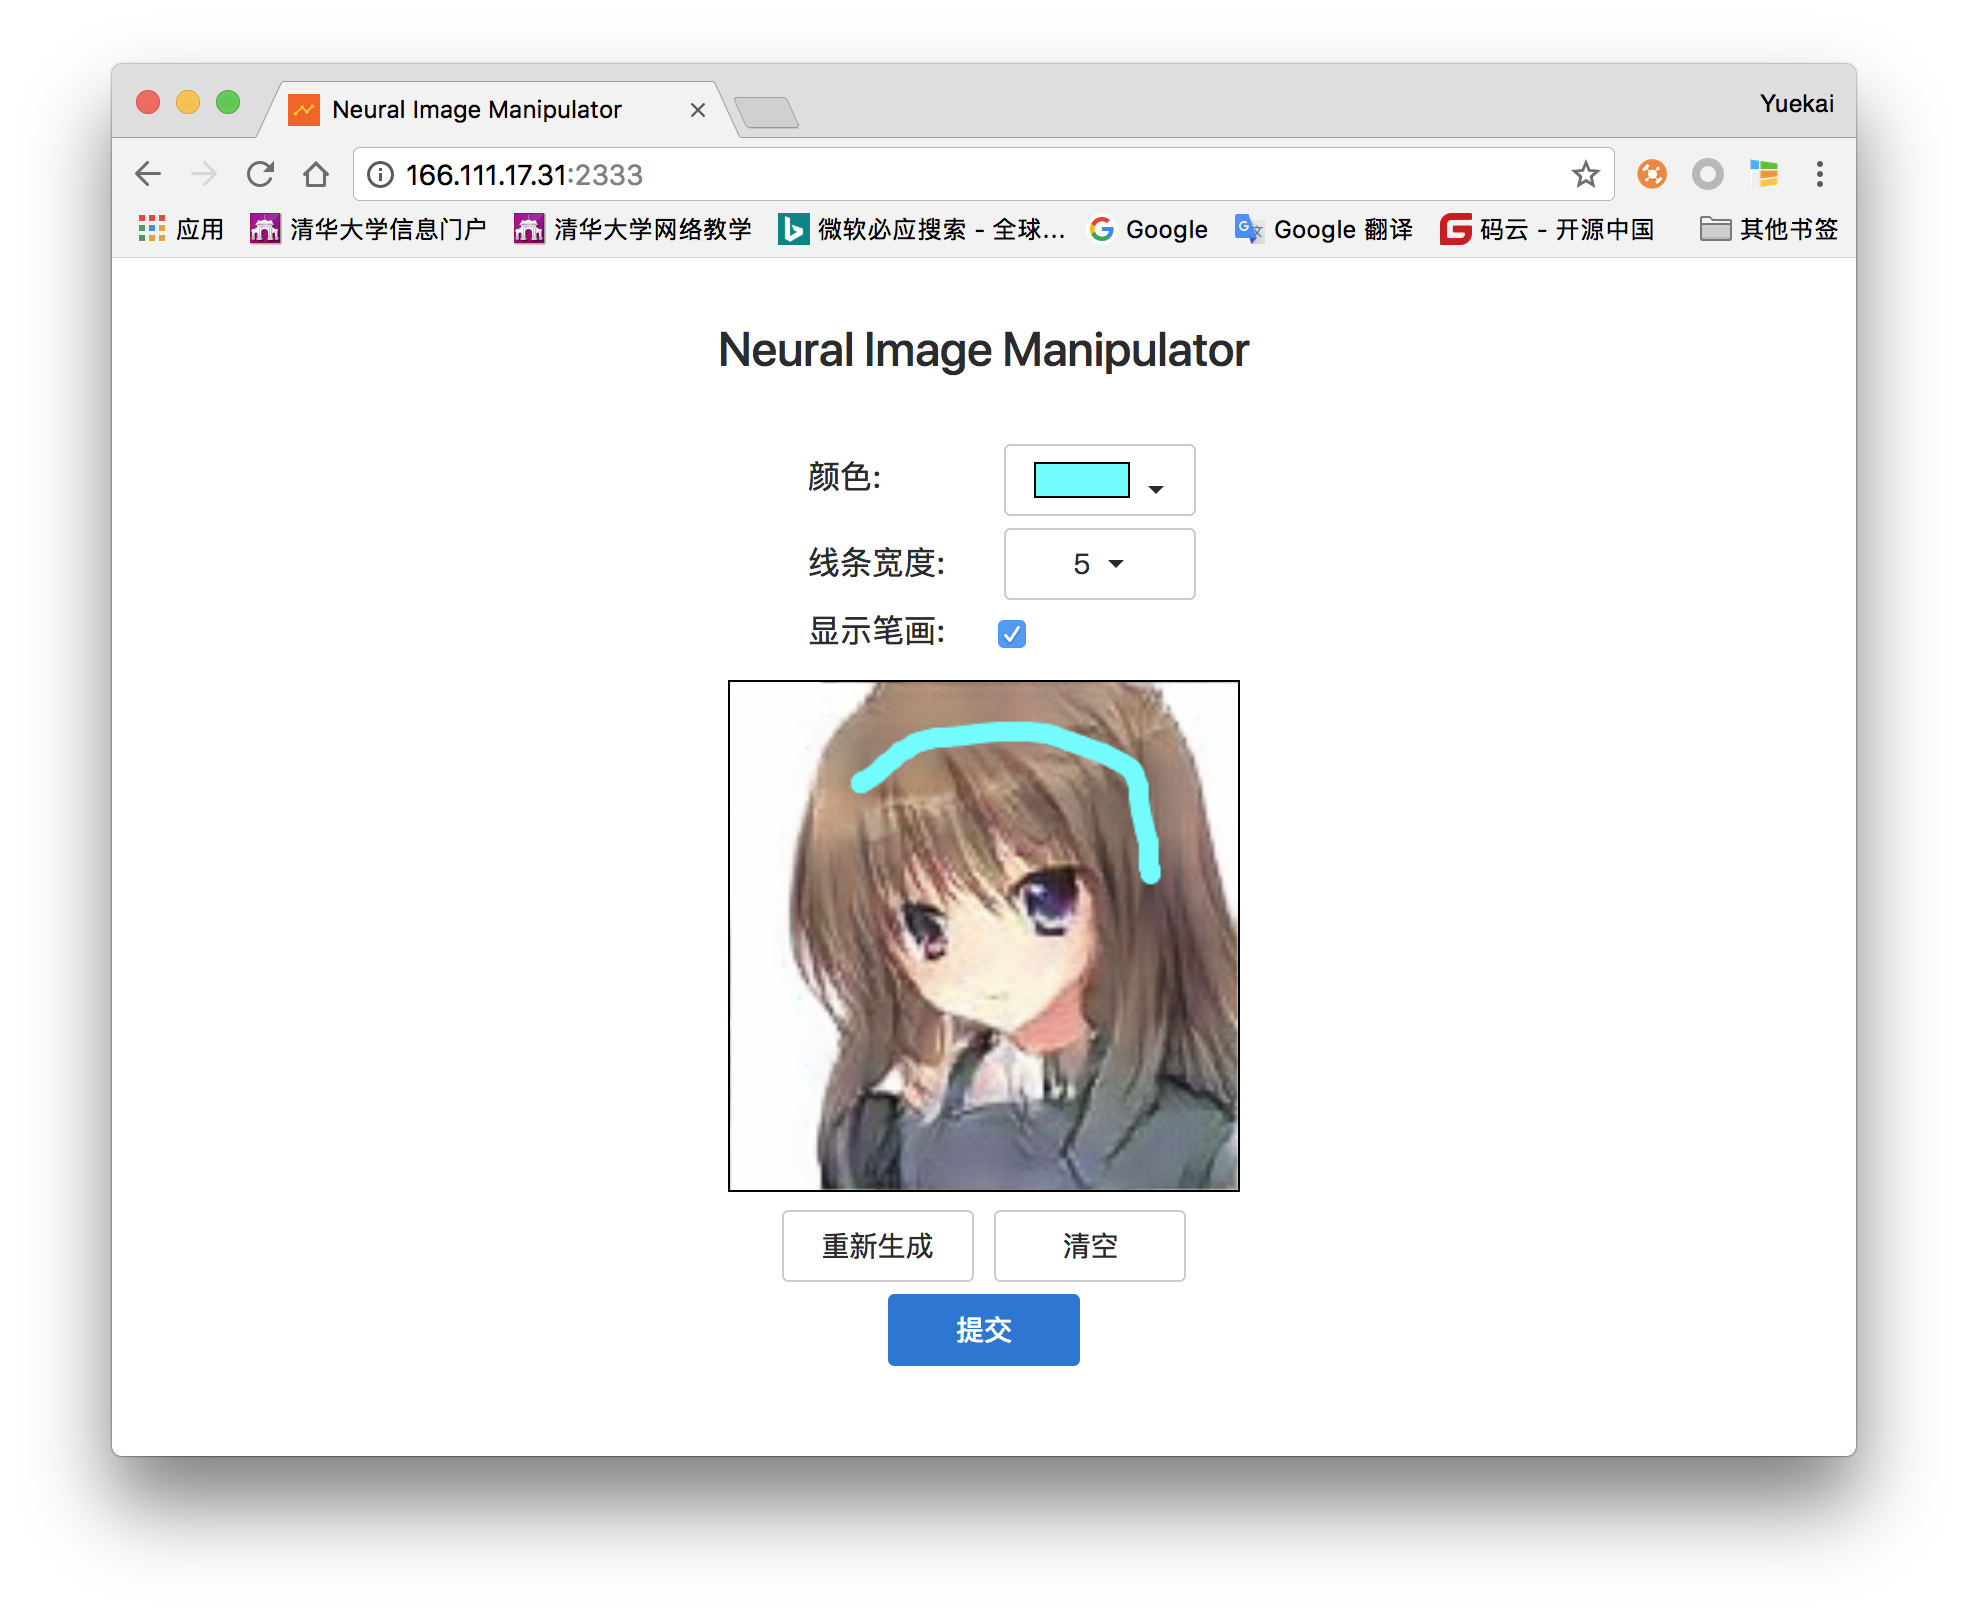
\includegraphics[height=4cm]{figs/web2.png}
      \caption{\kai 输入笔画}\label{figure:web2}
  \end{minipage}%
  \begin{minipage}[t]{0.33\linewidth}
      \centering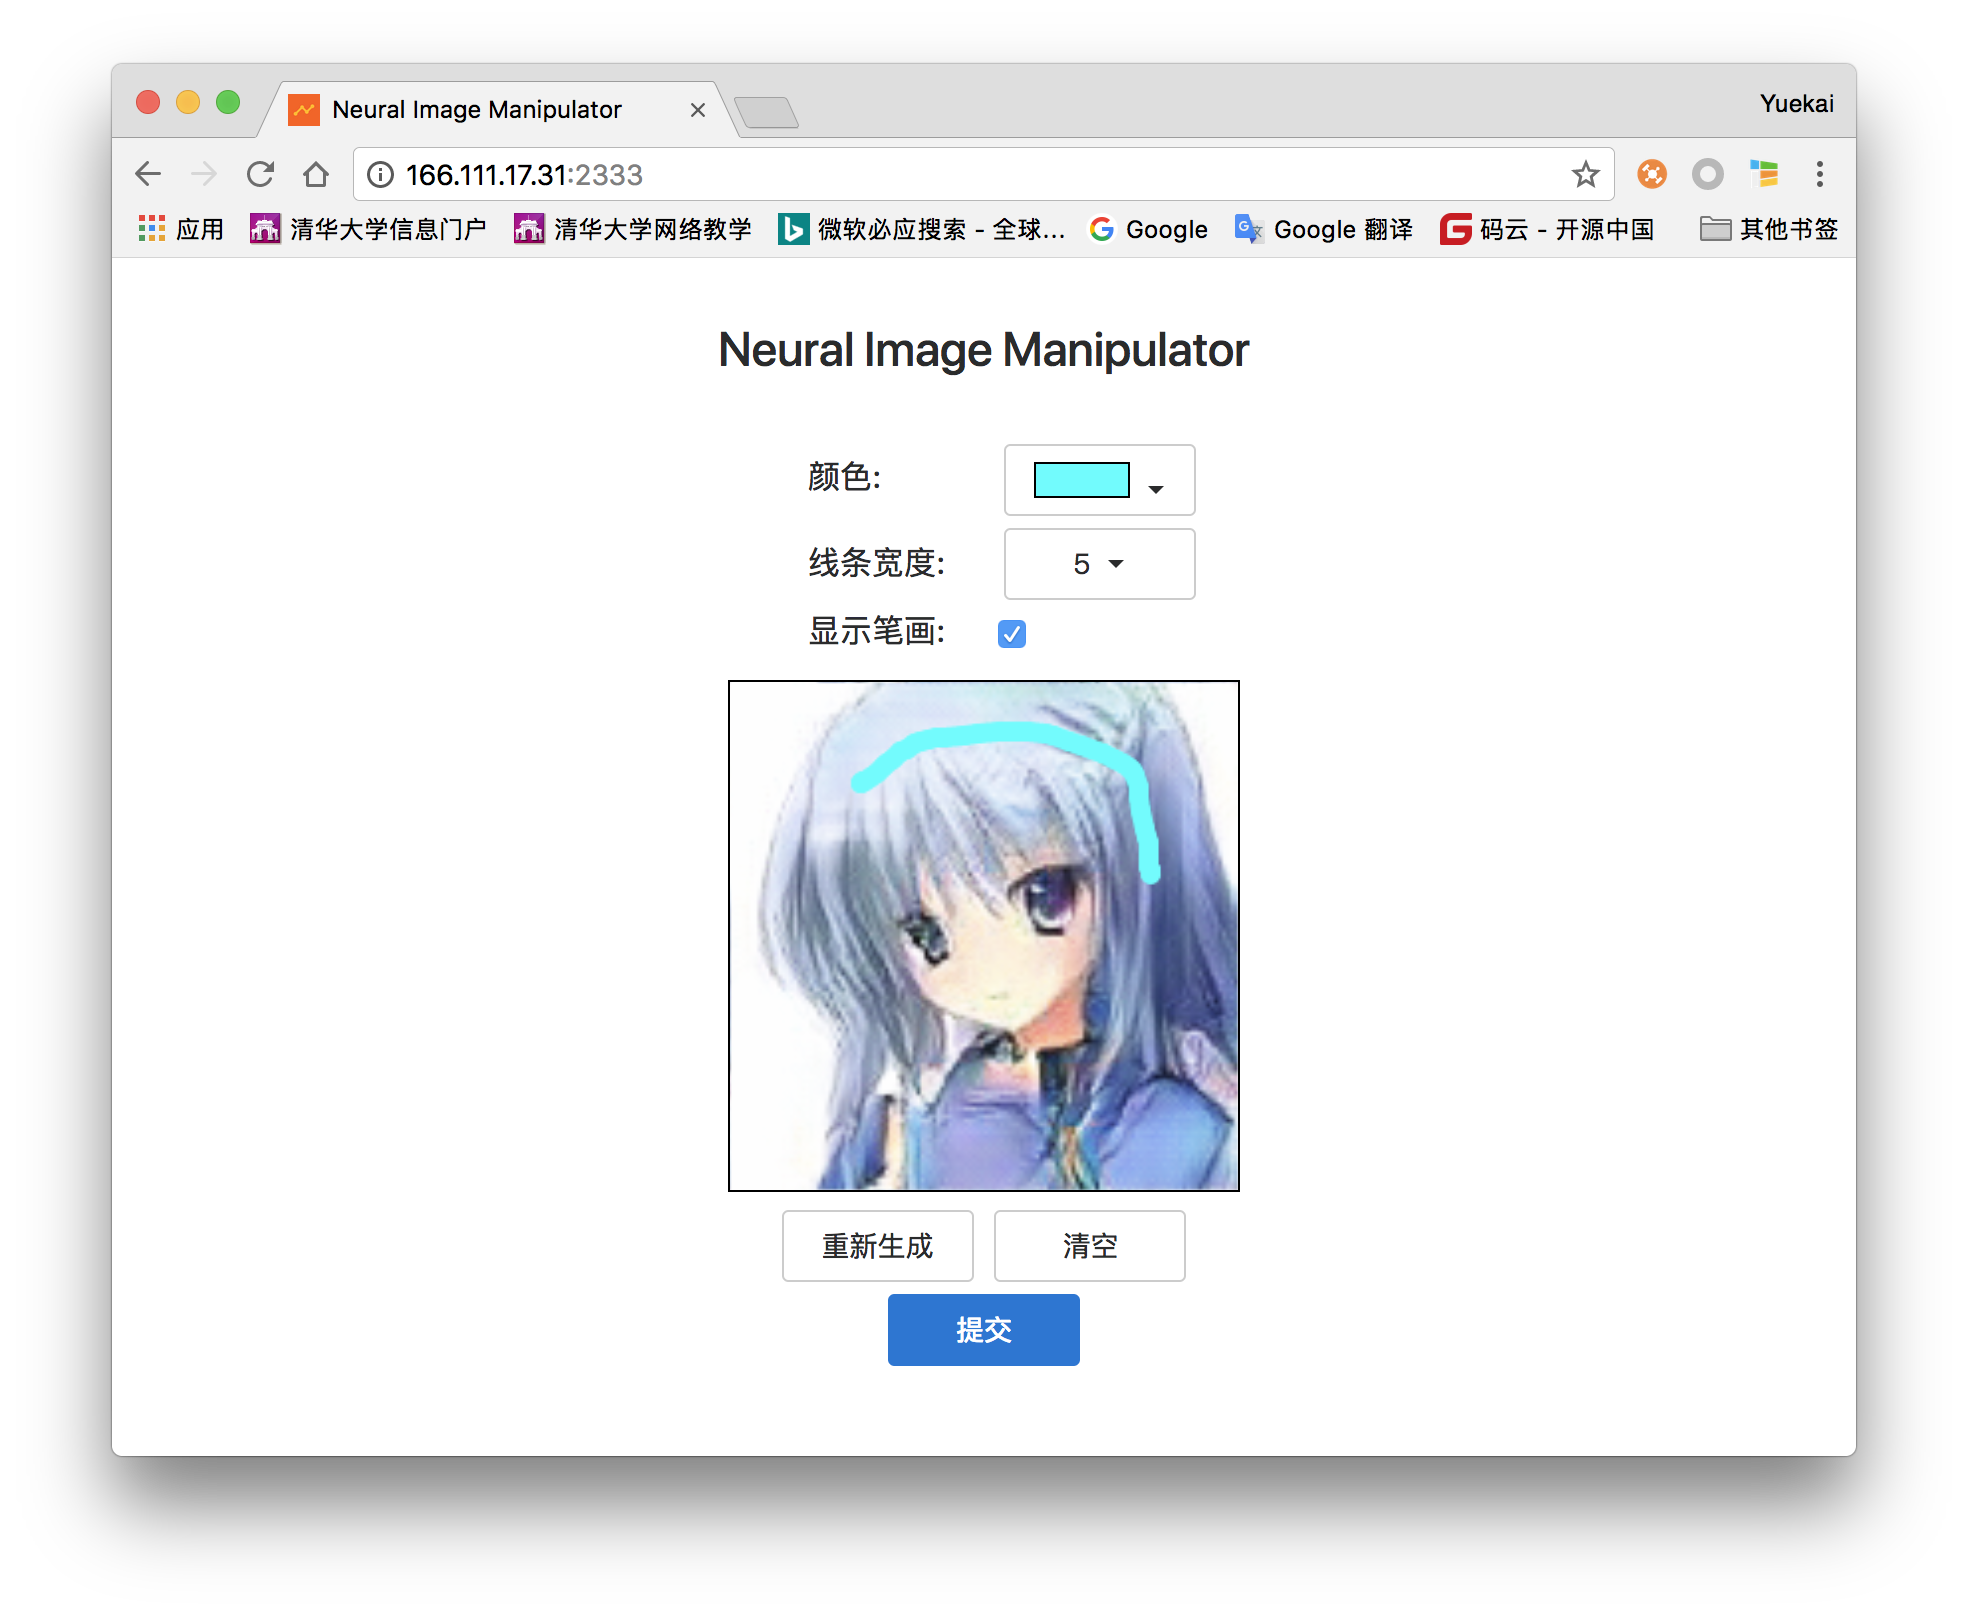
\includegraphics[height=4cm]{figs/web3.png}
      \caption{\kai 点击提交后}\label{figure:web3}
  \end{minipage}
\end{figure}

首次打开网页,点击 “开始按钮”,服务器会返回一张初始生成的图像。之后用户可以使用画笔工具,简单地勾勒出图片期望的变化方向,点击“提交”后,服务器就会返回在原图基础上,加上用户编辑条件后生成的图像;点击“重新生成”后,服务器会重新生成一张图片;点击“清空”能清空用户画的所有的笔画。此外,网页还支持更改画笔颜色、粗细,并能切换笔画的显示,以方便用户编辑。

该网页主要用 HTML 和 JavaScript 实现,并使用了 jQurey\footnote{\url{http://jquery.com}} 和 Bootstrap \footnote{\url{http://getbootstrap.com}} 等库。图片编辑框使用了 HTML5 的 \texttt{<canvas>},点击提交后,会将编辑框中的笔画图转成 Base64\footnote{\url{https://en.wikipedia.org/wiki/Base64}} 编码,使用 HTTP 请求发给服务器,之后服务器会返回生成图像的 Base64 编码,前端再将其作为图片编辑框的背景,显示给用户。

需要注意的是,用户每次点提交时,服务器是在该用户当前图像的基础上,再根据用户提供的笔画生成新图像,而且需要支持多用户同时编辑,即需要知道该用户当前的编辑状态。我们的做法是,服务器生成图像给前端时,会附带此时的 $z$ 和 $c$ 向量。前端将其保存下来,下次点提交时再发给服务器,服务器就会根据前端提供的 $z$ 和 $c$ 生成图像,以达到保存用户编辑状态的效果。

\subsubsection{服务器端}
由于训练模型使用的是 Python,所以我们选择了基于 Python 的 Django 框架搭建服务器端。

服务器端接收前端发来的笔画图,计算出 sketch 和 mask 矩阵,再根据前端发来的 $z$ 和 $c$,放入之前训练好的网络中,就能得到生成的图像。然后将其和修改后的 $z$ 和 $c$ 返回给前端。

实际测试时,模型的运行效率非常快,生成一张图像的时间仅需十几毫秒,主要延时在于网络传输。因此,就算是多个用户同时访问网页进行编辑,服务器也完全可以承受住这样的负载。

\section{结论}

本项目完成了神经图像编辑在动漫人脸数据集上的应用。我们尝试了多种模型与训练方法,找到了最佳的模型结构与参数,并实现了一个网页前端用于交互用户的编辑操作。与baseline方法相比较,我们的方法取得了如下的提升与贡献:

\begin{enumerate}
  \item 成功复现了高质量的动漫人物头像生成网络;
  \item 成功应用编辑图像方法于极深层的神经网络;
  \item 获得了高于基线的生成成果和编辑成果。包括生成真实度上升,生成清晰度上升($64 \times 64 \Rightarrow 128 \times 128$)和肉眼可见的编辑质量上升;
  \item 开发了基于B/S架构的网页应用。
\end{enumerate}

这次大作业,我们的收获主要有:
\begin{itemize}
  \item 通过对生成对抗网络(GAN)和 DCGAN、WGAN、DRAGAN 等变种的学习,对其原理和背后的思想有了更深的理解;
  \item 通过阅读大量论文,提升了文献阅读能力;
  \item 通过对大型网络模型的构建、训练与调参,对 TensorFlow 的使用更加熟练了,并锻炼了代码能力;
  \item 通过实现网页应用,学习了各种 Web 技术,并将神经网络模型成功转化为了实际产品;
  \item 通过小组合作开发,提升了团队协作能力,也从同组同学的身上学习到了许多新的知识。
\end{itemize}

\medskip

{\small
\bibliographystyle{ieee}
\bibliography{egbib}
}

\end{document}
